\section{Skill-R1: Agent Skill Evolution via Reinforcement Learning}
\label{sec:methodology}

We propose \textbf{Skill-R1} (illustrated in~\Cref{fig:flow}), a reinforcement learning framework that improves a frozen task model by recurrently refining external skills without updating the task model itself.
\textbf{Skill-R1} decouples \emph{task execution} from \emph{skill improvement}: a frozen task LLM generates rollout trajectories conditioned on a selected skill,
while a separate editor policy updates skills based on verified execution outcomes.


% \begin{figure}[H]
%     \centering
%     \includegraphics[width=\linewidth, height=4cm]{figures/phase1.pdf}
    
%     \includegraphics[width=\linewidth, height=4cm]{figures/phase2.pdf}
%     \caption{Overview of Skill-R1. \textbf{Phase 1} iteratively generates skills, rolls out a frozen task LLM, and stores verifier-scored outcomes in an evolutionary history. \textbf{Phase 2} computes a bi-level GRPO advantage from both intra-generation relative performance and inter-generation progress, and uses it to update the skill generator while keeping the task LLM frozen.}
%     \label{fig:flow}
% \end{figure}
\begin{figure}[ht]
\centering 
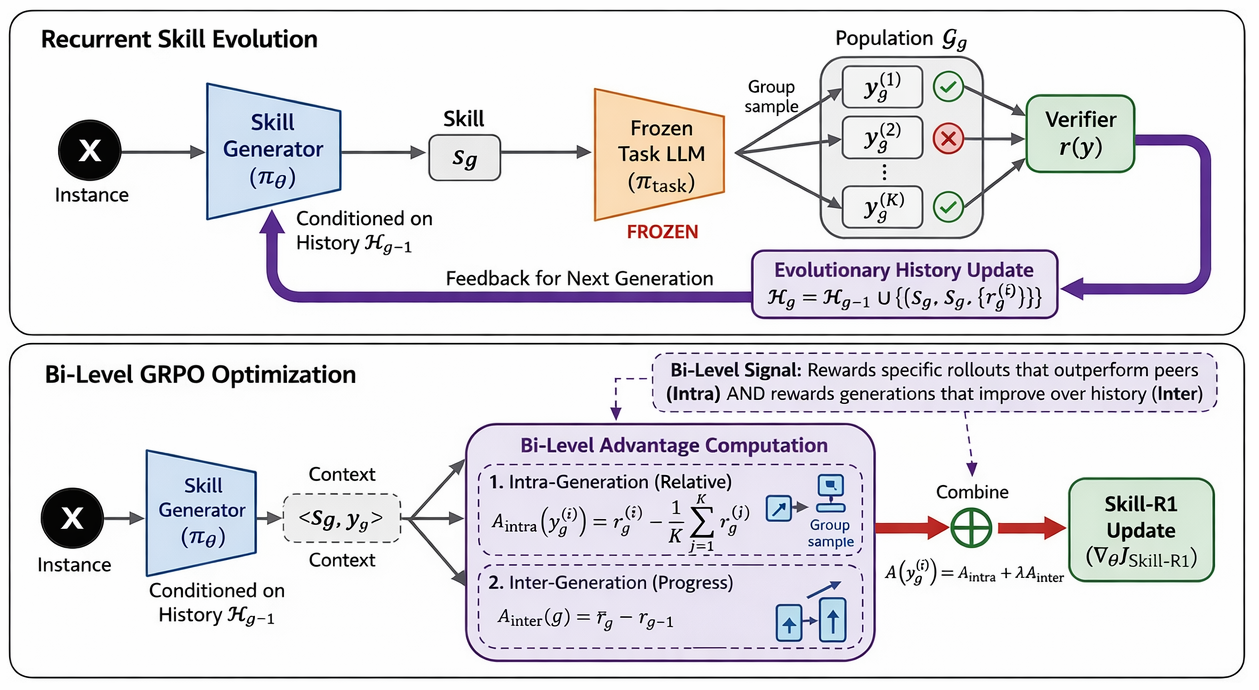
\includegraphics[width=1\linewidth]{figures/fig2-updated.png} 
\caption{Overview of Skill-R1. \textbf{Recurrent Skill Evolution} iteratively generates skills, rolls out a frozen task LLM, and stores verifier-scored outcomes in an evolutionary history. \textbf{Bi-level GRPO Optimization} computes GRPO advantages from both intra-generation relative performance and inter-generation progress, and uses it to update the skill generator while keeping the task LLM frozen.}
\label{fig:flow} 
\end{figure}

\subsection{Problem Setup} \label{sec:method-setup}

Let $x \in \mathcal{X}$ denote a task instance, and let $\mathcal{B}_x \subseteq \mathcal{S}$ denote the skill bank for instance $x$. 
Following \Cref{sec:prelim-skills}, for a selected skill $s_0 \in \mathcal{B}_{x}$, 
the frozen task model $\pi_{\mathrm{task}}$ induces a rollout distribution \Cref{eq:rollout_dist} over trajectories $y^{(i)} \in \mathcal{G}(x,s_0)$ group sampled (in \Cref{eq:group_sampling}) under skill conditioning, 
while a verifier $f_X:\mathcal{G}(x,s_0)\to\mathbb{R}$ assigns each rollout a scalar reward $r^{(i)}$. 
We also maintain the generation-wise history
\begin{equation} \label{eq:history_init}
\mathcal{H}_0 = \{(x, s_0,y^{(i)},r^{(i)})\}_{i=1}^{K},
\qquad 
y^{(i)} \sim \pi_{\mathrm{task}}(\cdot \mid x, s_0), 
\qquad
i=1,\dots,K.
\end{equation}
Thus, the instance-level performance induced by $s_0$ is determined by the rollout policy and verifier jointly,
and our goal is to improve performance on the given instance by revising skills so that later rollout populations achieve higher verifier reward.

For each generation $g \ge 1$, a learnable skill generator $\pi_\theta$ produces the next skill conditioned on the current instance and the accumulated history:
\begin{equation} \label{eq:skill_gen}
\tau = \{(s_g,\mathcal{G}_g(x,s_g),\{r_g^{(i)}\}_{i=1}^{K})\}_{g=1}^{G},
\qquad
s_g \sim \pi_\theta(\cdot \mid x, \mathcal{H}_{g-1}),
\qquad g=1,\dots,G.
\end{equation}
This defines a recurrent skill-evolution process in which each generated skill is evaluated through the rollout population it induces under the frozen task model \Cref{eq:rollout_dist}, 
and the resulting verifier outcomes are appended to the history to guide subsequent revisions. 
Then the recurrent skill evolution problem can be defined as optimizing $\pi_\theta$ to maximize verifier reward across the entire recurrent process:
\begin{equation} \label{eq:rl_objective}
J(\theta)
=
\mathbb{E}_{x \sim p(x)}
\mathbb{E}_{\substack{
s_g \sim \pi_\theta(\cdot \mid x, \mathcal{H}_{g-1}),\:
y_g^{(i)} \sim \pi_{\mathrm{task}}(\cdot \mid x, s_g)
}}
\left[
\sum_{g=1}^{G}
\gamma^{g-1}
\frac{1}{K}
\sum_{i=1}^{K} r_g^{(i)}
\right].
\end{equation}
Directly optimizing the objective in \eqref{eq:rl_objective} is challenging because the reward signal is evaluated on the task model's rollouts rather than directly on the generated skill. 
To address this structural decoupling between skill generation and task execution, we extend the standard GRPO framework to a bi-level setting. 
In the following section, we formulate a bi-level GRPO objective and derive \emph{bi-level advantages}. 
This formulation allows us to properly assign credit to the skill generator $\pi_\theta$ based on the relative, aggregate performance of the rollout populations that each skill induces.

% \todo[inline]{
% write about how we initialize the skill bank:
% In practice, the skill bank is initialized from a small seed set and then refined online. The episodic memory stores compact summaries of selected skills, rollout outcomes, mean rewards, and extracted success/failure patterns, and is shared by both the selector and the editor. The editor itself can operate in two modes: in \emph{inference mode}, the frozen task model proposes skill revisions from rollout evidence; in \emph{training mode}, a smaller trainable language model serves as the editor and provides token-level log-probabilities for policy optimization.
% }

% \todo[inline]{
% \textbf{MCMC interpretation of self-sampling.}
% A useful theoretical lens for the recurrent self-sampling process is Markov Chain Monte Carlo.
% For a fixed instance $x$, define the skill value
% \begin{equation}
% J(s;x) := \mathbb{E}_{y \sim \pi_{\mathrm{task}}(\cdot \mid x,s)}[\,r(y)\,],
% \label{eq:skill-value-main}
% \end{equation}
% and consider the associated energy-based target distribution over skills
% \begin{equation}
% p^\star_\beta(s \mid x) \propto \exp\!\big(\beta J(s;x)\big), \qquad \beta>0.
% \label{eq:skill-target-main}
% \end{equation}
% When $\beta$ is large, $p^\star_\beta(\cdot\mid x)$ concentrates on skills that maximize $J(s;x)$, which formalizes the notion of a ``best'' skill for the frozen task model on the current instance.
% In classical MCMC, one constructs a Markov chain whose stationary distribution equals $p^\star_\beta$ by using a proposal kernel and an acceptance rule that enforces detailed balance.
% While Skill-R1 does not explicitly implement an accept--reject mechanism, the target in
% \Cref{eq:skill-target-main} clarifies what it means for iterative self-sampling to concentrate on high-value skills.
% }

% \todo[inline]{
% \textbf{Stationary-limit and tracking bound.}
% Skill-R1 uses population rollouts to obtain Monte Carlo evidence about $J(s;x)$ and updates the skill proposal distribution
% $\pi_\phi$. Concretely, in generation $g$ the population mean reward
% \begin{equation}
% \widehat{J}_g := \frac{1}{K}\sum_{i=1}^K r\!\left(y^{(g,i)}\right)
% \label{eq:mc-estimator-main}
% \end{equation}
% estimates $J(s_g;x)$ for the sampled skill $s_g$, and the GRPO update increases the probability of proposing skills that
% yield larger $\widehat{J}_g$. Although $\phi$ changes across generations and the overall process is not a fixed-kernel MCMC,
% we can still make two precise statements.
% First, if the skill generator parameters converge, $\phi_g \to \phi^\star$, then the induced sampling distribution over
% skills becomes stationary at the limit, yielding a well-defined asymptotic proposal distribution for the instance.
% Second, when the parameter drift per generation is small, the induced sampling dynamics can be controlled by a tracking
% bound that quantifies how close the skill sampling distribution is to the stationary distribution of the corresponding
% frozen kernel. We formalize these statements and provide proof sketches in Appendix~\ref{app:mcmc_view}.
% }



\begin{algorithm}[ht]
\caption{Skill-R1: Agent Skill Evolution via Reinforcement Learning}
\label{alg:skillr1}
\begin{algorithmic}[1]
\Require Task distribution $p(x)$, frozen task LLM $\pi_{\mathrm{task}}$, skill generator $\pi_\theta$, initial skill bank $\mathcal{B}$, verifier $f$, generations $G$, group size $K$, mixing coefficient $\lambda$
\For{each task instance $x \sim p(x)$ and its skill bank $\mathcal{B}_x$}
    \State Select initial skill $s_0 \in \mathcal{B}_x$
    \State Sample rollouts $\mathcal{G}_0(x, s_0) = \{y_0^{(i)}\}_{i=1}^K$ from $\pi_{\mathrm{task}}(\cdot \mid x, s_0)$
    \State Score $r_0^{(i)} = f(y_0^{(i)})$ for each $i$; initialize $\mathcal{H}_0 = \{(x, s_0, y_0^{(i)}, r_0^{(i)})\}_{i=1}^K$
    \For{$g = 1, \dots, G$}
        \State Generate skill $s_g \sim \pi_\theta(\cdot \mid x, \mathcal{H}_{g-1})$ \Comment{\Cref{eq:skill_gen}}
        \State Sample rollouts $\mathcal{G}_g(x, s_g) = \{y_g^{(i)}\}_{i=1}^K$ from $\pi_{\mathrm{task}}(\cdot \mid x, s_g)$
        \State Verify $r_g^{(i)} = f(y_g^{(i)})$ for each $i$
        \State Compute $A_{\mathrm{intra}}(y_g^{(i)})$, $A_{\mathrm{inter}}(g)$, and $A(y_g^{(i)})$ \Comment{\Cref{eq:intra_adv,eq:inter_adv,eq:bilevel_adv}}
        \State Update $\mathcal{H}_g = \mathcal{H}_{g-1} \cup \{(s_g, \mathcal{G}_g, \{r_g^{(i)}\}_{i=1}^K)\}$
    \EndFor
\EndFor
\State Update $\theta$ by maximizing $\mathcal{L}_{\mathrm{Skill\text{-}R1}}(\theta)$ over accumulated rollouts \Comment{\Cref{eq:skillr1_obj}}
\end{algorithmic}
\end{algorithm}



\subsection{Bi-Level Group-relative Advantages }
\label{sec:method-advantage}

The reward signal in \Cref{eq:rl_objective} is evaluated on rollouts from the frozen task model, yet the trainable parameters reside in the skill generator $\pi_\theta$.
To route rollout-level feedback to the skill that induced it, we decompose credit assignment into two complementary advantage signals.
Within generation $g$, all $K$ rollouts share the same skill $s_g$, so we apply the group-relative comparison from \Cref{eq:grpo_adv} directly:
\begin{equation} \label{eq:intra_adv}
A_{\mathrm{intra}}(y_g^{(i)})
=
r_g^{(i)} - \frac{1}{K}\sum_{j=1}^K r_g^{(j)}.
\end{equation}
Centering by the group mean makes this signal invariant to absolute reward scale and isolates rollout quality from skill quality.
However, $A_{\mathrm{intra}}$ is blind to whether a skill revision improved on its predecessor.
To capture cross-generation progress, we define the population mean reward and the inter-generation advantage
\begin{equation} \label{eq:inter_adv}
A_{\mathrm{inter}}(g) = \bar{r}_g - \bar{r}_{g-1}, \qquad \bar{r}_g = \frac{1}{K}\sum_{i=1}^K r_g^{(i)}
\end{equation}
with $A_{\mathrm{inter}}(1)=0$.
A positive value indicates that the revised skill shifted the rollout distribution toward higher reward; a negative value penalizes regressions.
We combine the two signals into a single bi-level advantage:
\begin{equation}
A(y_g^{(i)}) = A_{\mathrm{intra}}(y_g^{(i)}) + \lambda\, A_{\mathrm{inter}}(g),
\label{eq:bilevel_adv}
\end{equation}
where $\lambda \ge 0$ interpolates between pure within-generation GRPO ($\lambda{=}0$) and a regime that additionally rewards cross-generation improvement.

\subsection{GRPO Objective for Skill Evolution}
\label{sec:method-objective}

We optimize $\pi_\theta$ with a clipped GRPO surrogate that aggregates the bi-level advantage across all generations.
Let $\rho_g = \pi_\theta(s_g \mid x, \mathcal{H}_{g-1}) / \pi_{\theta_{\mathrm{old}}}(s_g \mid x, \mathcal{H}_{g-1})$ be the importance ratio between the current and data-collection policies. The \textbf{Skill-R1} objective is
\begin{equation}
\begin{aligned}
\mathcal{L}_{\mathrm{Skill\text{-}R1}}(\theta)
&=
\mathbb{E}_{x \sim p(x)}
\Bigg[
\sum_{g=1}^{G}
\sum_{i=1}^{K}
\min\!\left(
  \rho_g\, A(y_g^{(i)}),\;
  \mathrm{clip}(\rho_g,\,1{-}\epsilon,\,1{+}\epsilon)\, A(y_g^{(i)})
\right)
\\
&\quad
-
\beta\,\mathrm{KL}\!\left(\pi_\theta(\cdot \mid x, \mathcal{H}_{g-1}) \,\|\, \pi_{\mathrm{ref}}(\cdot \mid x, \mathcal{H}_{g-1})\right)
\Bigg],
\end{aligned}
\label{eq:skillr1_obj}
\end{equation}
where $A(y_g^{(i)})$ is the bi-level advantage from \Cref{eq:bilevel_adv}, $\epsilon > 0$ is the clipping radius, and $\beta \ge 0$ weights a KL penalty anchoring the policy near a reference $\pi_{\mathrm{ref}}$.
% The clipped minimum stabilizes updates, while the KL term prevents degenerate collapse.
Summing over $g$ generations couples the objective across the entire recurrent process in \Cref{eq:skill_gen},
and thus $\pi_\theta$ is trained to produce improving skill trajectories rather than isolated single-step revisions.
Because only $\pi_\theta$ is updated, the task LLM $\pi_{\mathrm{task}}$ remains frozen and can be open- or closed-source and no gradients through $\pi_{\mathrm{task}}$ are required.
The full procedure is summarized in \Cref{alg:skillr1}.
